\achapter{20}{Products of Topological Spaces}\label{sec:Product_topology}


\vspace*{-17 pt}
\framebox{
\parbox{\dimexpr\linewidth-3\fboxsep-3\fboxrule}
{\begin{fqs}
\item What is the product of a finite number of topological spaces?
\item How do we define a topology on the product of a finite number of topological spaces?
\item What is a projection map from a product of a finite number of topological spaces? 
\item How can we use projection maps to determine the continuity of a function to a product of a finite number of topological spaces?
\item What is a subbasis of a topological space?
\item What properties do product spaces inherit from their factors?
\end{fqs}}}

\vspace*{13 pt}

\csection{Introduction}
In Section \ref{sec:metric_subspaces} we saw how we can make a Cartesian product of two metric spaces into a metric space. This is exactly the construction that allows us to work with the Cartesian plane $\R^2$ as a metric space with the usual metric. As we discussed in Section \ref{sec:top_spaces}, every metric space is a topological space, but not every topological space is metrizable. So knowing how to make a product of metric spaces into a metric space still leaves open the question of how we can make the product of topological spaces into a topological space. If we have two topological spaces $(X, \tau_X)$ and $(Y , \tau_Y)$, a natural approach to this problem might be to take as the open sets in $X \times Y$ the sets of the form $U \times V$ where $U \in \tau_X$  and $V \in \tau_Y$. We investigate this idea in Preview Activity \ref{PA:pd_top_1}.

\begin{pa} \label{PA:pd_top_1} Let $X = \{a,b,c\}$ with $\tau_X = \{\emptyset, \{a\}, \{b\}, \{a,b\}, \{a,c\}, X\}$, and let $Y = \{1,2\}$ with $\tau_Y = \{\emptyset, \{1\}, Y\}$. 
\be
\item Let 
\begin{equation} \label{eq:prod_basis}
\CB = \{U \times V \mid U \in \tau_X \text{ and } V \in \tau_Y\}.
\end{equation}
List all of the sets in $\CB$ along with their elements. 
 
\item Assume that all of the sets in $\CB$ are open sets in $X \times Y$. Should the set $A = \{(a,1), (a,2), (b,1)\}$ be an open set in $X \times Y$? Is the set $A$ of the form $U \times V$ for some open sets $U$ in $X$ and $V$ in $Y$? Explain. Is $\CB$ a topology on $X \times Y$? 

\item If $\CB$ is not a topology on $X \times Y$, what is the smallest collection of sets would we need to add to $\CB$ to make a topology on $X \times Y$? Explain your process. 

\ee

\end{pa}

\begin{comment}

\ActivitySolution

\be
\item  We take all products of open sets in $X$ and $Y$ to obtain the basis elements
\begin{align*}
\emptyset & \\
\{a\} \times \{1\} &= \{(a,1)\} \\
\{a\} \times Y &= \{(a,1), (a,2)\} \\
\{b\} \times \{1\} &= \{(b,1)\} \\
\{b\} \times Y &= \{(b,1), (b,2)\} \\
\{a,b\} \times \{1\} &= \{(a,1), (b,1)\} \\
\{a,b\} \times Y &= \{(a,1), (a,2), (b,1), (b,2)\} \\
\{a,c\} \times \{1\} &= \{(a,1), (c,1)\} \\
\{a,c\} \times Y &= \{(a,1), (a,2), (c,1), (c,2)\} \\
X \times \{1\} &= \{(a,1), (b,1), (c,1)\} \\
X \times Y &= \{(a,1), (a,2), (b,1), (b,2), (c,1), (c,2)\}.
\end{align*}

 
\item  We have $A = (\{a\} \times Y) \cup (\{b\} \times \{1\})$, so $A$ is a union of open sets in $X \times Y$ and should be open. But $A$ is not of the form $U \times V$ for some open sets $U$ in $X$ and $V$ in $Y$, as it is not in the list of those sets in part (a). 


\item Since $\CB$ is not closed under unions, $\CB$ is not a topology on $X \times Y$. However, if we consider all of the unions and finite intersections of sets in $\CB$ we create the topology 
\[\begin{array}{cccc}
\emptyset & \{(a,1)\} &\{(b,1)\} & \{(a,1), (a,2)\} \\
 \{(b,1), (b,2)\} & \{(a,1), (b,1)\} & \{(a,1), (c,1)\} & \{(a,1), (b,1), (b,2)\} \\
 \{(a,1), (a,2), (b,1)\} &\{(a,1), (a,2), (c,1)\} &  \{(a,1), (b,1), (c,1)\} & \{(a,1), (a,2), (b,1), (c,1)\} \\
 \{(a,1), (b,1), (b,2), (c,1)\} & \{(a,1), (a,2), (b,1), (b,2)\} & \{(a,1), (a,2), (b,1), (b,2), (c,1)\} & X \times Y  \end{array}\]
on $X \times Y$. In other words, we consider $\CB$ a basis for a topology of $X \times Y$. 

\ee

\end{comment}


\csection{The Topology on a Product of Topological Spaces} 

In our preview activity we learned that we cannot make a topology on a product $X \times Y$ of topological spaces $(X, \tau_X)$ and $(Y , \tau_Y)$ with just the sets of the form $U \times V$ where $U \in \tau_X$ and $V \in \tau_Y$ as the open sets since the collection of these sets is not closed under arbitrary unions. What we can do instead is consider these unions of all of the sets of the form $U \times V$, where $U$ is open in $X$ and $V$ is open in $Y$. In other words, consider these sets to be a basis for the topology on $X \times Y$. 

\begin{activity} \label{act:box_topology} Let $(X, \tau)$ and $(Y, \tau_Y)$ be topological spaces, and let $\CB$ be as defined in (\ref{eq:prod_basis}). Prove that $\CB$ is a basis for a topology on $X \times Y$.

\end{activity}

\begin{comment}

\ActivitySolution Since $X \in \tau_X$ and $Y \in \tau_Y$, every point in $X \times Y$ is in a set in $\CB$. So $\CB$ satisfies condition 1 of a basis. Suppose $(x,y) \in (U_1 \times V_1) \cap (U_2 \times V_2)$. Then $x \in U_1 \cap U_2$ and $y \in V_1 \cap V_2$, and 
\[(x,y) \in (U_1 \cap U_2) \times (V_1 \cap V_2) \subseteq (U_1 \times V_1) \cap (U_2 \times V_2).\]
So $\CB$ is a basis for a topology on $X \times Y$. 

\end{comment}

The argument from Activity \ref{act:box_topology} can be extended to a product of any finite number of topological spaces. Let $n$ be a positive integer and let $(X_i, \tau_i)$ be topological spaces for $i$ from $1$ to $n$. Let 
\[\CB = \left\{ \Pi_{i=1}^n O_i \mid O_i \text{ is open in } X_i\right\}.\]
 Since $X_i \in \tau_i$ for every $i$, every point in $\Pi_{i=1}^n X_i$ is in a set in $\CB$. So $\CB$ satisfies condition 1 of a basis. Now we show that $\CB$ satisfies the second condition of a basis.  Let $B_1 = \Pi_{i=1}^n U_i$ and $B_2 = \Pi_{i=1}^n V_i$ for some open sets $U_i$, $V_i$ in $X_i$. Suppose $(x_i) \in (B_1 \cap B_2)$. Then for each $j$ we have $x_j \in U_j \cap V_j$ and so
\[(x_i) \in \Pi_{i=1}^n (U_i \cap V_i).\]
Since $U_i \cap V_i$ is an open set in $X_i$, it follows that $\Pi_{i=1}^n (U_i \cap V_i)$ is in $\CB$. Thus, $\CB$ is a basis for a topology on $X \times Y$. 

This topology generated by products of open sets is called the \emph{box} or \emph{product} topology.

\begin{definition} \label{def:box_topology} Let $(X_{\alpha}, \tau_{\alpha})$ be a collection of topological spaces for $\alpha$ in some finite indexing set $I$. The \textbf{box topology}\index{box topology} or \textbf{product topology}\index{product topology} on the product $\Pi_{\alpha \in I} X_{\alpha}$ is the topology with basis
\[\CB = \left\{ \Pi_{\alpha \in I} U_{\alpha} \mid U_{\alpha} \in \tau_{\alpha}  \text{ for each } \alpha \in I \right\}.\]
\end{definition}

So we can always make the product of topological spaces into a topological space using the box topology. 

\csection{Three Examples}

In this section we consider three specific examples of a product of topological spaces. 

\begin{activity} Let $X = [1,2]$ and $Y = [3,4]$ as subspaces of $\R^2$. 
\ba
\item Explain in detail what the product space $X \times Y$ looks like. 

\item Find, if possible, an open subset of $X \times Y$ that is not of the form $U \times V$ where $U$ is open in $X$ and $V$ is open in $Y$.

\ea

\end{activity}

\begin{comment}

\ActivitySolution

\ba
\item The product space $X \times Y$ contains all points of the form $(x,y)$ with $1 \leq x \leq 2$ and $3 \leq y \leq 4$ in $\R^2$. This set of points is the rectangle in $\R^2$ with vertices $(1,3)$, $(2,3)$, $(1,4)$ and $(2,4)$. 

\item The set $O = \{(x,y) \mid 1.1 < x < 1.3, 3.1 < y < 3.3\} \cup \{(x,y) \mid 1.7< x < 1.9, 3.7 < y < 3.9\}$ is equal to $(B(1.2,0.1) \times B(3.2,0.1)) \cup ((B(1.8,0.1) \times B(3.8,0.1))$ and so is open in $X \times Y$. However, $O$ is not of the form $U \times V$ where $U$ is open in $X$ and $V$ is open in $Y$. To see why, suppose to the contrary that $O = U \times V$ for some $U$ open in $X$ and $V$ open in $Y$. Since the points $(x,y)$ in $O$ only have $x \in (1.1,1.3) \cup (1.7,1.9)$ and $y \in (3.1,3.3) \cup (3.7,3.9)$, it follows that $U = (1,1,1.3) \cup (1.7,1.9)$ and $V = (3.1,3.3) \cup (3.7,3.9)$. But then $(1.8, 3.2)$ is in $U \times V$. Since $(1.8, 3.2)$ is not in $O$, we conclude that $O$ is not of the for $U \times V$ with $U$ open in $X$ and $V$ open in $Y$.  

\ea


\end{comment}


\begin{activity} Let $X = \R$ and $Y = S^1 = \{(x,y) \mid x^2 + y^2 = 1\}$, the unit circle as a subset of $\R^2$.  
\ba
\item Draw a picture of $\R$. For each $x \in \R$, the set $\R_x = \{(x, y) \mid y \in S^1\}$ is a subset of $\R \times S^1$. On your graph of $\R$, draw pictures of $\R_x$ for $x$ equal to $-1$, $0$, and $1$. Explain in detail what the product space $\R \times S^1$ looks like. 

\item Consider the sets of the form $B \cap S^1$, where $B$ is an open ball in $\R^2$ (relatively open sets in $S^1$). What do these sets look like?

\item Describe the shape of the basis elements for the product topology on $\R \times S^1$ that result from products of the form $U \times V$, where $U$ is an open interval in $\R$ and $V$ is the intersections of $S^1$ with an open ball in $\R^2$. 

\ea

\end{activity}

\begin{comment}

\ActivitySolution

\ba
\item We draw $\R$ as a horizontal line. At each point $x$ on the line, we draw a circle or radius 1 on the line as shown at left in Figure \ref{F:Product_example_tube} for $x=-1$, $x=0$, and $x=1$. The complete product space looks like an infinitely long tube as shown at right in Figure \ref{F:Product_example_tube} . 
\begin{figure}[h]
\begin{center}
\resizebox{!}{1.2in}{\includegraphics[trim=1.25cm 2.25cm 1.25cm 2.5cm, clip]{Product_example_tube_1.png}} \hspace{0.2in} \resizebox{!}{1.2in}{\includegraphics[trim=1.25cm 2.25cm 1.25cm 2.5cm, clip]{Product_example_tube_2.png}}
\caption{Left: $R_x$ for $x$ equal to $-1$, $0$, and $1$. Right: The product space.} 
\label{F:Product_example_tube}
\end{center}
\end{figure}
%\includegraphics[trim=left bottom right top, clip]{file}

\item When we intersect an open ball with a circle, we get an open arc on the circle. 

\item If we cross an open interval in $\R$ with an open arc on the circle, the resulting figure looks like a finite length trough as depicted in Figure \ref{F:Tube_open}. 
\begin{figure}[h]
\begin{center}
\resizebox{!}{1.2in}{\includegraphics[trim=1.25cm 2.25cm 1.25cm 3.0cm, clip]{Product_example_tube_3.png}} 
\caption{An example $U \times V$.} 
\label{F:Tube_open}
\end{center}
\end{figure}
%\includegraphics[trim=left bottom right top, clip]{file}
\ea

\end{comment}

\begin{activity} Let $2S^1 = \{(x,y) \mid x^2 + y^2 = 4\}$ be the circle of radius $2$ centered at the origin as a subset of $\R^2$. In this activity we investigate the space $2S^1 \times  S^1$.  
\ba
\item Draw a picture of $2S^1$ in the $xy$-plane. For each $p \in S^1$, the set $S^1_p = \{(p, y) \mid y \in S^1\}$ is a subset of $S^1 \times S^1$. On your graph of $S^1$, draw pictures of $S^1_p$ for $p$ equal to $(1,0)$, $\left(\frac{\sqrt{2}}{2}, \frac{\sqrt{2}}{2}\right)$, and $(0,1)$. Orient the graphs so that the copies of $S^1$ are perpendicular to $2S^1$. Explain in detail what the product space $2S^1 \times S^1$ looks like. 

\item Consider the sets of the form $B \cap S^1$, where $B$ is an open ball in $\R^2$. What do these sets look like?

\item Describe the shape of the basis elements for the product topology on $2S^1 \times S^1$ that result from products of the form $U \times V$, where $U$ and $V$ are intersections of $S^1$ with open balls in $\R^2$. 

\ea

\end{activity}

\begin{comment}

\ActivitySolution

\ba
\item A picture of $2S^1$ and $S^1_p = \{(p, y) \mid y \in S^1\}$ for $p$ equal to $(1,0)$, $\left(\frac{\sqrt{2}}{2}, \frac{\sqrt{2}}{2}\right)$, and $(0,1)$ are shown at left in Figure \ref{F:Product_example_torus}. The product space $2S^1 \times S^1$ looks like a torus as illustrated at right in Figure \ref{F:Product_example_torus}.
\begin{figure}[h]
\begin{center}
\resizebox{!}{1.0in}{\includegraphics[trim=1.25cm 2.0cm 1.25cm 2.0cm, clip]{Product_example_torus_1.png}} \hspace{0.5in} \resizebox{!}{1.0in}{\includegraphics[trim=1.25cm 2.0cm 1.25cm 2.0cm, clip]{Product_example_torus_2.png}}
\caption{Left: Cross sections of the product space. Right: The product space. $2S^1 \times S^1$.} 
\label{F:Product_example_torus}
\end{center}
\end{figure}
%\includegraphics[trim=left bottom right top, clip]{file}

\item When we intersect an open ball with a circle, we get an open arc on the circle. 

\item We cross an open arc on $2S^1$ with an open arc on $S^1$ and the result is a slice of the torus both horizontally and vertically as illustrated in Figure \ref{F:Torus_open}.
\begin{figure}[h]
\begin{center}
\resizebox{!}{1.0in}{\includegraphics[trim=1.25cm 1.25cm 1.25cm 2.0cm, clip]{Product_example_torus_3.png}}
\caption{An example $U \times V$ on $2S^1 \times S^1$.} 
\label{F:Torus_open}
\end{center}
\end{figure}
\ea

\end{comment}

\csection{Projections and Continuous Functions on Products}

Given topological spaces $(X_1, \tau_1)$ and $(X_2, \tau_2)$, we define $\pi_1: X_1 \times X_2 \to X_1$ and $\pi_2: X_1 \times X_2 \to X_2$  by $\pi_1((x,y)) = x$ and $\pi_2((x,y)) = y$. These functions $\pi_1$ and $\pi_2$ are the \emph{projections}\index{projection functions} of $X_1 \times X_2$ onto $X_1$ and $X_2$, respectively. These projection functions can help us determine when a function $f$ from a topological space $Y$ to $X_1 \times X_2$ is continuous.

\begin{activity} \label{act:projection_continuous} Let $(X_1, \tau_1)$ and $(X_2, \tau_2)$ be topological spaces and let $O_1$ be an open set in $X_1$. 
\ba
\item Determine which set is $\pi_1^{-1}(O_1)$. Verify your conjecture.

\item Explain why $\pi_1$ is continuous.

\ea

\end{activity}

\begin{comment}

\ActivitySolution

\ba
\item We will demonstrate that $\pi_1^{-1}(O_1) = O_1 \times X_2$. Let $(s,t) \in \pi_1^{-1}(O_1)$. Then $\pi_1((s,t)) = s \in O_1$. So $(s,t) \in O_1 \times X_2$ and $\pi_1^{-1}(O_1) \subseteq O_1 \times X_2$. Now let $(s,t) \in O_1 \times X_2$. Then $\pi_1((s,t)) = s \in O_1$ and $(s,t) \in \pi_1^{-1}(O_1)$. 

\item Recall that the sets $O_1 \times O_2$ with $O_1 \in \tau_1$ and $O_2 \in \tau_2$ form a basis for the product topology. Part (a) shows that the inverse image of an open set in $X_1$ under $\pi_1$ is open in $X_1 \times X_2$, so we conclude that $\pi_1$ is a continuous function.

\ea

\end{comment}

The same argument as in Activity \ref{act:projection_continuous} shows that $\pi_2$ is also a continuous function. In general, if $X = \Pi_{i=1}^n X_{i}$ is a finite product of topological spaces, then the projection $\pi_{k}: X \to X_{k}$ is a continuous function for each $k$, where $\pi_k((x_1,x_2, \ldots, x_n)) = x_k$. %We note here that there is another topology, called the \emph{product topology}\index{product topology}) on $X$ with subbasis $S = \bigcup S_{\alpha \in I} S_{\alpha}$, where 
%\[S_{\alpha} = \{\pi_{\alpha}^{-1}(U_{\alpha}) \mid U_{\alpha} \text{ is open in } X_{\alpha}\}.\] 
%For reasons we won't go into, the product topology is preferred to the box topology for infinite products (many important theorems that hold for finite products will not hold for infinite products using the box topology, but will hold using the product topology). However, the product topology and the box topology are the same for finite products, and since we won't consider infinite products here we will not worry about the distinction. For our purposes we will use the terms ``box topology" and ``product topology" interchangeably.

Let $O = \Pi_{i=1}^n O_i$ be a basic open set in $X = \Pi_{i=1}^n X_i$, where $X_i$ is a topological space for each $i$. We can extend the result of Activity \ref{act:projection_continuous} to see that
\[\pi_i^{-1}(O_i) = X_1 \times X_2 \times \cdots \times X_{i-1} \times O_i \times X_{i+1} \times \cdots \times X_n.\]
So 
\[\Pi_{i=1}^n O_i = \bigcap_{i=1}^n \pi_i^{-1}(O_i).\]
So each basic open set is a finite intersection of sets of the form $\pi_i^{-1}(O_i)$ where $O_i$ is open in $X_i$. When this happens, we call the collection of sets of the form $\pi_i^{-1}(O_i)$ a \emph{subbasis} of the topology. 

\begin{definition} \label{def:subbasis} Let $(X, \tau)$ be a topological space. A subset $\CS$ of $\tau$ is a \textbf{subbasis}\index{subbasis} or \textbf{subbase}\index{subbase} for $\tau$ if the set of all finite intersections of elements of $\CS$ is a basis for $\tau$. 
\end{definition}

As an example, since finite intersections of intervals of the form $(-\infty,b)$ and $(a, \infty)$ give all intervals of the form $(a,b)$, the collection $\CS = \{(-\infty,b), (a, \infty) \mid a, b \in \R\}$ is a subbasis for the standard topology on $\R$. Note that this collection itself is not a basis for the standard topology on $\R$. If $X = \Pi_{i=1}^n X_i$ is a product of topological space, then another example of a subbasis is the collection
\[\CS = \bigcup_{i=1}^n \{\pi_i^{-1}(O_i) \mid O_i \text{ is open in } X_i\}.\]
This set is a subbasis for the product topology on $X$ (the verification of this is left to Exercise (\ref{ex:subbasis})). 

We note here that there is another topology, called the \emph{product topology}\index{product topology}) on $X$ with subbasis $S = \bigcup S_{\alpha \in I} S_{\alpha}$, where 
\[S_{\alpha} = \{\pi_{\alpha}^{-1}(U_{\alpha}) \mid U_{\alpha} \text{ is open in } X_{\alpha}\}.\] 
For reasons we won't go into, the product topology is preferred to the box topology for infinite products (many important theorems that hold for finite products will not hold for infinite products using the box topology, but will hold using the product topology). However, the product topology and the box topology are the same for finite products, and since we won't consider infinite products here we will not worry about the distinction. For our purposes we will use the terms ``box topology" and ``product topology" interchangeably.

As we have discussed before, it can often be easier to define a topology using a basis or subbasis than it is to describe all of the sets in the topology. As we might expect, since the continuity of a function can be determined by the inverse image of basis elements, the continuity of a function can also be determined by the inverse image of subbasis elements.

\begin{activity} Prove Theorem \ref{thm:subbasis_continuous}. (Hint: Recall that $f$ is continuous if $f^{-1}(B)$ is open in $X$ for each basic open set $B$.)

\begin{theorem} \label{thm:subbasis_continuous} Let $(X, \tau_X)$ and $(Y, \tau_Y)$ be topological spaces, let $\CS$ be a subbasis for $\tau_Y$, and let $f: X \to Y$ be a function. If $f^{-1}(S)$ is open in $X$ for each $S \in \CS$, then $f$ is continuous.
\end{theorem}

 \end{activity}

\begin{comment}

\ActivitySolution Recall that $f$ is continuous if $f^{-1}(B)$ is open in $X$ for each basic open set $B$. Let $B$ be a basic open set. Since $\CS$ is a subbasis for $\tau_Y$, there are finitely many elements $S_1$, $S_2$, $\ldots$, $S_n$ in $\CS$ such that $B = \bigcap_{i=1}^n S_i$. Then
\[f^{-1}(B) = f^{-1}\left( \bigcap_{i=1}^n S_i \right) = \bigcap_{i=1}^n f^{-1}(S_i).\]
Because $f^{-1}(S_i)$ is open in $X$ for each $i$, and any finite intersection of open sets is open, we conclude that $f^{-1}(B)$ is open in $X$ and that $f$ is continuous.

\end{comment}

Now suppose that $X_1$, $X_2$, and $Y$ are topological spaces, and that $f: Y \to X_1 \times X_2$ is a function. Then $\pi_1 \circ f$ maps $Y$ to $X_1$ and $\pi_2 \circ f$ maps $Y$ to $X_2$. Since the composition of continuous functions is continuous, we can see that if $f$ is continuous so are $\pi_1\circ f$ and $\pi_2 \circ f$. To determine if $f$ is a continuous function, it would be useful to know if the converse is true. A key idea in the proof is the result of Exercise (\ref{ex:inverse_composite_sets}) on page \pageref{ex:inverse_composite_sets} that if $R$, $S$, and $T$ are sets, and $g: R \to S$ and $h : S \to T$ are functions, then $(h \circ g)^{-1}(O) = g^{-1}(h^{-1}(O)$ for any subset $O$ of $T$.  


%\begin{activity} Let $X_1$, $X_2$, and $Y$ be topological spaces, and let $f: Y \to X_1 \times X_2$ be a function.  Assume that $\pi_1\circ f$ is continuous. Let $O_1$ be an open set in $X_1$. Show that $(\pi_1\circ f)^{-1}(O_1) = f^{-1}(\pi_1^{-1}(O_1)$.  

%\end{activity}

%\begin{comment}

%\ActivitySolution First let $(x_1,x_2) \in (\pi_1\circ f)^{-1}(O_1)$. Then $(\pi_1 \circ f)((x_1,x_2)) \in O_1$. It follows that $\pi_1(f((x_1,x_2)) \in O_1$. So $f((x_1,x_2)) \in \pi_1^{-1}(O_1)$. From this we have $(x_1,x_2) \in f^{-1}(\pi_1^{-1}(O_1))$. We conclude that $(\pi_1\circ f)^{-1}(O_1) \subseteq f^{-1}(\pi_1^{-1}(O_1))$. 

%Now suppose that $(x_1,x_2) \in f^{-1}(\pi^{-1}(O_1))$. Then $f((x_1,x_2)) \in \pi_1^{-1}(O-1)$. From this we have that $\pi_1(f((x_1,x_2))) \in O_1$. Thus, $(\pi_1 \circ f)((x_1,x_2)) \in O_1$ and $(x_1,x_2) \in (\pi_1\circ f)^{-1}(O_1)$. We conclude that $f^{-1}(\pi_1^{-1}(O_1)) \subseteq (\pi_1\circ f)^{-1}(O_1) $. The two containments verify the equality $(\pi_1\circ f)^{-1}(O_1) = f^{-1}(\pi_1^{-1}(O_1))$.

%\end{comment}

Now we can use projections to determine when functions to product spaces are continuous.

\begin{theorem} \label{thm:prod_continuity} Let $X_i$ for $i$ from $1$ to $n$ and $Y$ be topological spaces, and let $f: Y \to \Pi_{i=1}^n X_i$ be a function. Then $f$ is continuous if and only if $\pi_i \circ f$ is continuous for each $i$. 
\end{theorem}

\begin{proof} Let $X_i$ for $i$ from $1$ to $n$ and $Y$ be topological spaces, and let $f: Y \to \Pi X_i$ be a function. If $f$ is continuous, the facts that each $\pi_i$ is continuous and that composites of continuous functions are continuous show  that $\pi_i \circ f$ is continuous for each $i$. 

Now suppose that $\pi_i \circ f$ is continuous for each $i$. Recall that 
\[\CS = \{\pi_i^{-1}(O_i) \mid O_i \text{ is open in } X_i\}\]
is a subbasis for the product topology on $\Pi_{i=1}^n X_i$. To prove that $f$ is continuous, Theorem \ref{thm:subbasis_continuous} tells us that it is enough to show that $f^{-1}(S)$ is open for each $S$ in $\CS$. Let $O_i$ be an open set in $X_i$. Exercise (\ref{ex:inverse_composite_sets}) on page \pageref{ex:inverse_composite_sets} tells us that 
\[f^{-1}(\pi_i^{-1}(O_i)) = (\pi_i \circ f)^{-1}(O_i),\]
which is open in $Y$ because $\pi_i \circ f$ is continuous. Therefore, $f$ is continuous.  
\end{proof}
 
\csection{Properties of Products of Topological Spaces}

It is natural to ask what topological properties of the topological spaces $(X, \tau_X)$ and $(Y, \tau_Y)$ are inherited by the product $X \times Y$. We have studied Hausdorff, connected, and compact spaces, and we now consider those properties. 

\begin{activity} Let $(X, \tau_X)$ and $(Y, \tau_Y)$ be Hausdorff spaces.
\ba
\item What will it take to prove that the space $X \times Y$ with the product topology is Hausdorff?

\item Suppose that $(x_1,y_1), (x_2, y_2) \in X \times Y$. What does the fact that $X$ is Hausdorff tell us about $x_1$ and $x_2$? What can we say about $y_1$ and $y_2$?

\item Complete the proof of the following theorem.

\begin{theorem} If $(X, \tau_X)$ and $(Y, \tau_Y)$ are Hausdorff spaces, then $X \times Y$ with the product topology is a Hausdorff space. 
\end{theorem}

\ea

\end{activity}

\begin{comment}

\ActivitySolution

\ba
\item We need to show that if $a = (x_1,y_1)$ and $b = (x_2,y_2)$ are distinct points in $X \times Y$, then there are disjoint open sets $U$ and $V$ in $X \times Y$ such that $a \in U$ and $b \in V$. 

\item The fact that $X$ is Hausdorff tells us that there exist open sets $U_1$ and $U_2$ in $X$ such that $x_1 \in U_1$, $x_2 \in U_2$, and $U_1 \cap U_2 = \emptyset$. Similarly, the fact that $Y$ is Hausdorff tells us that there exist open sets $V_1$ and $V_2$ in $Y$ such that $y_1 \in V_1$, $y_2 \in V_2$, and $V_1 \cap V_2 = \emptyset$.

\item From part (b) we know that $(x_1,y_1) \in U_1 \times V_1$ and $(x_2, y_2) \in U_2 \times V_2$, and 
\[(U_1 \times V_1) \cap (U_2 \times V_2) = (U_1 \cap U_2) \times (V_1 \cap V_2) = \emptyset.\]
So the sets $U_1 \times V_1$ and $U_2 \times V_2$ separate $(x_1,y_1)$ and $(x_2, y_2)$ and $X \times Y$ is a Hausdorff space. 

\ea

\end{comment}

The proofs that a product of connected spaces is connected, that a product of path connected spaces is path connected, and that a product of compact spaces is compact are a bit more complicated. To prove that a product of two connected spaces is connected, we will use the result of Activity \ref{act:connected_compenent} in Section \ref{sec:Connected_topology} that the union of connected subsets is connected if the intersection of the subsets is nonempty. A consequence of this result is the following.
\label{cor:Connected_union}
\begin{lemma} \label{lem:Connected_union} Let $X$ be a topological space, and let $A_{\alpha}$ be a connected subset of $X$ for all $\alpha$ in some indexing set $I$. Let $B$ be a connected subset of $X$ such that $A_{\alpha} \cap B \neq \emptyset$ for every $\alpha \in I$. Then $B \cup \left(\bigcup_{\alpha \in I} A_{\alpha} \right)$ is connected. 
\end{lemma}

\begin{proof} Let $X$ be a topological space, and let $A_{\alpha}$ be a connected subset of $X$ for all $\alpha$ in some indexing set $I$. Let $B$ be a connected subset of $X$ such that $A_{\alpha} \cap B \neq \emptyset$ for every $\alpha \in I$. For each $\alpha \in I$ let $B_{\alpha} = B \cup A_{\alpha}$. Let $\beta \in I$. Since $B \cap A_{\beta} \neq \emptyset$, Lemma \ref{lem:Connected_union} shows that $B_{\beta}$ is connected. Given that $B$ is not empty, and $B \subseteq \bigcap_{\alpha \in I} B_{\alpha}$, we see that $\bigcap_{\alpha \in I} B_{\alpha} \neq \emptyset$. Lemma \ref{lem:Connected_union} allows us to conclude that $\bigcup_{\alpha \in I} B_{\alpha}$ is connected. But 
\[\bigcup_{\alpha \in I} B_{\alpha} = \bigcup_{\alpha \in I} (B \cup A_{\alpha}) = B \cup \left(\bigcup_{\alpha \in I} A_{\alpha}\right),\]
and so $B \cup \left(\bigcup_{\alpha \in I} A_{\alpha}\right)$ is connected. 
\end{proof}

We will use Lemma \ref{lem:Connected_union} to show that a product of connected spaces is connected. 
 
\begin{theorem} \label{thm:connected_product} If $(X, \tau_X)$ and $(Y, \tau_Y)$ are connected topological spaces, then $X \times Y$ with the product topology is a connected topological space.  
\end{theorem}

\begin{proof} Assume $(X, \tau_X)$ and $(Y, \tau_Y)$ are connected topological spaces. Our approach to proving that $X \times Y$ is connected is to write $X \times Y$ as a union of two connected subspaces whose intersection is not empty. Let $a \in X$. The space $X_a = \{a\} \times Y$ is homeomorphic to $Y$ via the inclusion map $i$ which sends $(a,t) \in \{a\} \times Y$ to the point $t \in Y$. Since $Y$ is connected, so is $X'$. Let $b \in Y$. The space $Y_b = X \times \{b\}$ is homeomorphic to $X$ via the inclusion map $i$ which sends $(s,b) \in X \times \{b\}$ to the point $s \in X$. Since $X$ is connected, so is $Y_b$. (The verification of these homeomorphisms is left to the reader.) The point $(a,b)$ is in $X_a \cap Y_b$, so $X_a \cap Y_b \neq \emptyset$ for every $b \in Y$. It follows that $X_a \cup \left( \bigcup_{t \in Y} Y_t \right)$ is connected by Lemma \ref{lem:Connected_union}. All that remains is to prove that $X_a \cup \left( \bigcup_{t \in Y} Y_t \right) = X \times Y$ and we will have demonstrated that $X \times Y$ is connected.  The fact that $X_a \subseteq X \times Y$ and $Y_t \subseteq X \times Y$ for every $t \in Y$ implies that $X_a \cup \left( \bigcup_{t \in Y} Y_t \right) \subseteq X \times Y$. It then remains to show that $X \times Y \subseteq X_a \cup \left( \bigcup_{t \in Y} Y_t \right)$. Let $(u,v) \in X \times Y$. Then $u \in X$ and $v \in Y$ and $(u,v) \in Y_v$. Thus, $X \times Y \subseteq X_a \cup \left( \bigcup_{t \in Y} Y_t \right)$ and so $X \times Y = X_a \cup \left( \bigcup_{t \in Y} Y_t \right)$. Therefore, $X \times Y$ is connected.  
\end{proof}

Once we know that a product of connected topological spaces is connected, we can extend that result to any finite number of connected spaces by induction.

\begin{corollary} Let $X_{k}$ be a connected topological space for $k$ from 1 to $n$. Then the product $\Pi_{k=1}^n X_k$ is connected.
\end{corollary}

The proof is left to Exercise (\ref{ex:connected_product}). 

We conclude this section by demonstrating that a product of compact topological spaces is compact. It is also true that finite products of path connected and compact spaces are path connected and compact. The proofs are left to Exercises (\ref{ex:compact_product}) and (\ref{ex:path_connected_product}). 
 
\begin{theorem} \label{thm:compact_product} If $X$ and $Y$ are compact topological spaces, then $X \times Y$ is a compact topological space under the product topology.
\end{theorem}
 
\begin{proof} Let $(X, \tau_X)$ and $(Y, \tau_Y)$ be compact topological spaces. Let $\CC = \{O_{\alpha}\}$ be an open cover of $X \times Y$ for $\alpha$ in some indexing set $I$. Let $a \in X$ and let $Y_a = \{a\} \times Y$. Since $Y_a$ is homeomorphic to $Y$, we know that $Y_a$ is compact. The collection $\{O_{\alpha} \cap Y_a\}$ is an open cover of $Y_a$, and so has a finite sub-cover $\{O_{\alpha_i}\}_{1 \leq i \leq n}$. The set $N_a = \bigcup_{1 \leq i \leq n} O_{\alpha_i}$ is an open set that contains $Y_a$. We will show that there is a neighborhood $W_a$ of $a$ that $N_a$ contains the entire set $W_a \times Y$. 

Cover the set $Y_a$ with open sets that are contained in $N_a$ (since $N_a$ is open, we can intersect any open set with $N_a$ and still have an open set). Each open set is a union of basis elements, so we can cover $Y_a$ with basis elements $U \times V$ that are contained in $N_a$. Since $Y_a$ is compact, there is a finite collection $U_1 \times V_1$, $U_2 \times V_2$, $\ldots$, $U_m \times V_m$ of basis elements contained in $N_a$ that cover $Y_a$. Assume that each $U_i \times V_i$ intersects $Y_a$ (otherwise, we can remove that set and still have a cover). Let $W_a = U_1 \cap U_2 \cap \cdots \cap U_m$.  Since $a \in U_i$ for each $i$, we know that $W_a$ is not empty. Each $U_i$ is open in $X$ and so $W_a$ is open in $X$. Thus, $W_a$ is a neighborhood of $a$ in $X$. Now we demonstrate that $W_a \times Y \subseteq \bigcup_{1 \leq i \leq m} U_i \times V_i$. Let $(x,y) \in W_a \times Y$. Since the collection $\{U_i \times V_i\}_{1 \leq i \leq m}$ covers $Y_a$, the point $(a,y)$ is in $U_k \times V_k$ for some $k$ between $1$ and $m$. So $y \in Y_k$.  But $x \in W_a = \bigcap_{1 \leq i \leq m} U_i$, so $x \in U_k$. Thus, $(x,y) \in U_k \times V_k$ and we conclude that $W_a \times Y \subseteq \bigcup_{1 \leq i \leq m} U_i \times V_i$.

So for each $a \in X$, the set $N_a$ contains a set of the form $W_a \times Y$, where $W_a$ is a neighborhood of $a$ in $X$. So $W_a \times Y$ is covered by a finite sub-cover of our open cover $\CC$ of $X \times Y$. The collection $\{W_a \times Y\}_{a \in X}$ is an open cover of $X \times Y$. Since $X$ is compact, the is a finite sub-cover $W_1$, $W_2$, $\ldots$, $W_r$ of the open cover $\{W_a\}_{a \in X}$ of $X$. is an open cover of $X$. It follows that the sets $W_1 \times Y$, $W_2 \times Y$, $\ldots$, $W_r \times Y$ is a cover of $X \times Y$. For each $i$, the set $W_i \times Y$ is covered by finitely many of the sets in $\CC$, and so the collection of these sets forms a finite sub-cover of $X \times Y$ in $\CC$. Therefore, $X \times Y$ is compact. 
\end{proof}

\csection{Summary}
Important ideas that we discussed in this section include the following. Throughout, let $(X_i, \tau_i)$ be topological spaces for $i$ from $1$ to some integer $n$
\begin{itemize}
\item The product of the $X_i$ is the Cartesian product $\Pi_{i=1}^n X_i$. 
\item The set 
\[\CB = \left\{ \Pi_{i=1}^n O_i \mid O_i \text{ is open in } X_i\right\}\]
 is a basis for the box topology on $\Pi_{i=1}^n X_i$. 
\item The mapping $\pi_j : \Pi_{i=1}^n X_i \to X_j$ defined by $\pi_j((x_i)) = x_j$ is the projection map onto $X_j$ for $j$ from 1 to $n$. 
\item A function $f$ mapping a topological space $Y$ to $\Pi_{i=1}^n X_i$ is continuous if and only if $\pi_j \circ f$ is continuous for every $j$ from $1$ to $n$. 
\item Let $(X, \tau)$ be a topological space. A subset $\CS$ of $\tau$ is a subbasis for $\tau$ if the set $\CS$ of all finite intersections of elements of $\CS$ is a basis for $\tau$. 
\item If each $X_i$ is (a) connected, (b) path connected, (c) compact, then $\Pi_{i=1}^n X_i$ is (a) connected, (b) path connected, (c) compact with respect to the product topology.
\end{itemize}

\csection{Exercises}

\be

\item \label{ex:subbasis}
\ba

\item Let $(Y_1, \tau_1)$ and $(Y_2, \tau_2)$ be topological spaces, where $Y_1 = \{a,b,c\}$ with $\tau_1 = \{\emptyset, \{a\}, \{b,c\}, Y_1\}$ and $Y_2 = \{1,2\}$ with $\tau_2 = \{\emptyset, \{1\}, Y_2\}$. Find all of the sets of the form 
\[\CS = \{\pi_1^{-1}(O_1) \mid O_1 \text{ is open in } Y_1\} \cup \{\pi_2^{-1}(O_2) \mid O_2 \text{ is open in } Y_2\}\]
and verify that these sets generate the product topology on $Y_1 \times Y_2$. 

\item Let $X_{i}$ for $i$ from $1$ to $n$ be topological spaces and let $X = \Pi_{i=1}^n X_i$. Show that the collection
\[\CS = \bigcup_{i=1}^n \{\pi_i^{-1}(O_i) \mid O_i \text{ is open in } X_i\}\]
is a subbasis for the box topology on $X$. 

\ea

\begin{comment}

\ExerciseSolution 

\ba

\item The product topology on $Y_1 \times Y_2$ is 
\[\{\emptyset, \{a\} \times \{1\}, \{b,c\} \times \{1\}, Y_1 \times \{1\}, \{a\} \times Y_2, \{b,c\} \times Y_2, Y_1 \times Y_2\}.\]

Now 
\begin{align*}
\pi_1^{-1}(\{a\}) &= \{(a,1), (a,2)\} = \{a\} \times Y_2 \\
\pi_1^{-1}(\{b,c\}) &= \{(b,1), (b,2), (c,1), (c,2)\} = \{b,c\} \times Y_2 \\ 
\pi_1^{-1}(Y_1) &= Y_1 \times Y_2 \\
\pi_2^{-1}(\{1\}) &= \{(a,1), (b,1), (c,1)\} = Y_1 \times \{1\},
\end{align*}
and so $\CS = \{\emptyset, \{a\} \times Y_2, \{b,c\} \times Y_2, Y_1 \times \{1\}, Y_1 \times Y_2\}$. The collection of finite intersections of elements of $\CS$ is $\{\emptyset, \{a\} \times \{1\}, \{a\} \times Y_2, \{b,c\} \times \{1\}, \{b,c\} \times Y_2, Y_1 \times \{1\}\}$. Since $(\{a\} \times Y_2) \cup (\{b,c\} \times Y_2) = Y_1 \times Y_2$, we see that $\CS$ is a subbasis for the product topology on $Y_1 \times Y_2$.  

\item Let $\tau$ be the box topology on $X$ and $\tau'$ the topology generated by the elements in $\CS$. Because each $\pi_i$ is continuous, the elements $\pi_i^{-1}(O_i)$ where $O_i$ is open in $X_i$ are all open sets, So every element in $\CS$ is in $\tau$ and $\tau' \subseteq \tau$. We will next demonstrate that $\Pi_{i=1}^n O_i = \bigcap_{i = 1}^n \pi_i^{-1}(O_i)$. This will show that every set in $\tau$ is also in $\tau'$ and so $\tau = \tau'$. 

Let $x = (x_i) \in \Pi_{i=1}^n O_i$. So $x_i \in O_i$ for each $i$ and $x \in \pi_i^{-1}(O_i)$ for each $i$. It follows that $\Pi_{i=1}^n O_i \subseteq \bigcap_{i = 1}^n \pi_i^{-1}(O_i)$. Now let $(x_i) \in \bigcap_{i = 1}^n \pi_i^{-1}(O_i)$. Then $x_i = \pi_i(x) \in O_i$ for each $i$. So $x \in \Pi_{i=1}^n O_i$. Thus, $\bigcap_{i = 1}^n \pi_i^{-1}(O_i) \subseteq \Pi_{i=1}^n O_i$ and we conclude that $\Pi_{i=1}^n O_i \subseteq \bigcap_{i = 1}^n \pi_i^{-1}(O_i)$. So the collection of finite intersections of elements of $\CS$ forms the product topology and we conclude that $\CS$ is a subbasis for the product topology. 

\ea

\end{comment}


\item Let $X$ be the set of real numbers with the standard Euclidean metric topology and let $Y$ be the real numbers with the discrete topology. 

	\ba
	\item Explain why the set of all ``horizontal intervals" of the form 
	\[I= (a,b) \times \{c\} = \{(x,c) \mid a < x < b\}\]
	is a base for the product topology on $X \times Y$.
	
	\item Find the interior and closure of each of the following subsets of $X \times Y$.
	
		\begin{enumerate}
		\item $A = \{(x,0) \mid 0 \leq x < 1\}$
		
		\item $B = \{(0,y) \mid 0 \leq y < 1\}$ 
		
		\item $C = \{(x,y) \mid 0 \leq x < 1, 0 \leq y < 1\}$
		
		\end{enumerate}
	
	\ea
	
\begin{comment}

\ExerciseSolution

\ba

\item The open sets in $X$ are generated by the open intervals $(a,b)$ with $a < b$ while the open sets in $Y$ are generated by the singleton sets. Thus, the basic open sets in $X \times Y$ have the form $(a,b) \times \{c\}$ for some $a < b$ in $\R$ and some $c \in \R$. This gives the set $I = \{(x,c) \mid a < x < b\}$. 

\item 
	\begin{enumerate}[i.]
	\item There is no open interval of the form $(a,b)$ that contains $0$ without having $a < 0$. So $(0,0)$ cannot be contained in an open set entirely contained in $A$. If $0 < x < 1$, then $(x,0) \in (0,x+0.5|1-x|) \times \{0\} \subseteq A$. So every point except $(0,0)$ is an interior point of $A$ and $\Int(A) = \{(x,0) \mid 0 < x < 1\}$. 
	
	We know that $\overline{A} = A \cup A'$, so it suffices to find the limit points of $A$ that are not in $A$. The neighborhood $(x-1,x+1) \times \{y\}$ does not intersect $A$ if $y \neq 0$, so no points of the form $(x,y)$ with $y \neq 0$ are in $A'$. Similarly, the neighborhood $(x-r,x+r) \times \{0\}$ with $r = 0.5\min\{|x|, |1-x|\}$ does not intersect $A$ if $x > 1$ or $x < 0$. Finally, the neighborhoods of the point $(1,0)$ all contain a basic open set of the form $(a,b) \times \{0\}$ with $a < 0 < b$, and each of these basic open sets contains a point in $A$. Thus, $(1,0) \in A'$. We conclude that $\overline{A} = \{(x,0) \mid 0 \leq x \leq 1\}$.
	
	\item There is no basic open set $I = (a,b) \times \{c\}$ that is entirely contained in $B$, so $\Int(B) = \emptyset$.  
	
The neighborhood $(x-r, x+r) \times \{0\}$ where $r = 0.5|x|$ does not intersect $B$ if $x \neq 0$, so no points of the form $(x,y)$ with $x \neq 0$ are in $B'$. Similarly, the neighborhood $(x-1,x+1) \times \{y\}$ of the point $(x,y)$ does not intersect $B$ if $y \geq 1$ or $y < 0$. We conclude that $\overline{B} = B$. 
	
	\item If $0 < x,y < 1$, then the basic open set $(x-r, x+r) \times \{y\}$ with $r = \min\{|x|, |1-x|\}$ is entirely contained in $C$, so every point of the form $(x,y)$ with $0 < x,y < 1$ is in the interior of $C$. Every open set that contains a point of the form $(0,y)$ for $0 \leq y < 1$ must contain a basic open set $(a,b) \times \{y\}$ with $a < 0 < b$. But none of these neighborhoods is contained in $C$, so $\Int(C)$ contains no points $(x,y)$ with $x = 0$. Finally, if $0 < x < 1$, then the neighborhood $(x-r, x+r) \times \{y\}$ with $r = \min\{|x|, |1-x|\}$ is entirely contained in $C$ and so these points are in the interior of $C$. We conclude that $\Int(C) = \{(x,y) \mid 0 < x < 1, 0 \leq y < 1\}$. 
	
The neighborhood $(x-1,x+1) \times \{y\}$ of the point $(x,y)$ does not intersect $C$ if $y \geq 1$ or $y < 0$, so points of this form are not in $C'$. Similarly, the neighborhood $(x-r,x+r) \times \{y\}$ with $r = 0.5\min\{|x|, |1-x|\}$ does not intersect $C$ for any value of $y$ if $x > 1$ or $x < 0$. So points of this form are not in $C'$. Any neighborhood of the point $(0,y)$ for $0 \leq y < 1$ contains a basic open set of the form $(a,b) \times \{y\}$ with $a < 0 < b$, and each of these basic open sets contains a point in $C$. So these points are all limit points of $C$. Along those same lines, any neighborhood of the point $(1,y)$ for $0 \leq y < 1$ contains a basic open set of the form $(a,b) \times \{y\}$ with $a < 1 < b$, and each of these basic open sets contains a point in $C$. So these points are all limit points of $C$. We conclude that $\overline{C} = \{(x,y) \mid 0 \leq x \leq 1, 0  \leq y < 1\}$. 
	
	\end{enumerate}

\ea

\end{comment}

\item \label{ex:product_closure} Let $X_1$ and $X_2$ be topological space and let $A_1$ be a subset of $X_1$ and $A_2$ a subset of $X_2$. Assume the product topology on $X_1 \times X_2$. Prove each of the following.

\ba

\item $\overline{A_1 \times A_2} = \overline{A_1} \times \overline{A_2}$

\item $\Int(A_1 \times A_2) \subseteq \Int{A_1} \times \Int{A_2}$

\ea

\begin{comment}

\ExerciseSolution

\ba

	\item  Let $x = (x_1, x_2) \in \overline{A_1 \times A_2}$. We demonstrate that $x_i \in \overline{A_i}$ for each $i$.  Let $O_i$ be an open set in $X_i$ that contains $x_i$. The projection map $\pi_i$ is continuous, so $\pi_i^{-1}(O_i)$ is open in $X_1 \times X_2$. Since $x \in \overline{A_1 \times A_2}$, every open set that contains $x$ contains a point in $A_1 \times A_2$. So $\pi_i^{-1}(O_i)$ contains a point $t = (t_1,t_2)$ in $A_1 \times A_2$. But then $\pi_i(t) = t_i$ is in $O_i$ and $t_i \in A_i$. Thus every open neighborhood of $x_i$ contains a point in $A_i$. We conclude that $x_i \in \overline{A_i}$ and $\overline{A_1 \times A_2} \subseteq \overline{A_1} \times \overline{A_2}$. 	
	
Now suppose that $x = (x_1,x_2) \in \overline{A_1} \times \overline{A_2}$. Let $U$ be an open set that contains $x$ in $X_1 \times X_2$. Then $U$ contains a basis element $U_1 \times U_2$ that contains $x$. The fact that $x_1 \in \overline{A_1}$ and $x_2 \in \overline{A_2}$ implies that there is an element $x_1' \in U_1 \cap A_1$ and an element $y_1' \in U_2 \cap A_2$. Then $(x_1',y_1') \in U$ and $(x_1', y_1') \in A_1 \times A_2$. Thus, every open set that contains $x$ also contains a point $(x_1',y_1')$ in $A_1 \times A_2$. So $x \in \overline{A_1 \times A_2}$.  
	
		
	\item  Suppose $x = (x_1,x_2) \in \Int(A_1 \times A_2)$. Then there is an open set $U$ in $A_1 \times A_2$ such that $x \in U$. The fact that $U$ is open means that $U$ is a union of basic open sets, so there is a basic open set $U_1 \times U_2$ that is contained in $A_1 \times A_2$ that contains $x$. So $x_1 \in U_1$ and $x_2 \in U_2$. But $U_i \subset A_1$, so each $x_i$ is in $\Int(A_i)$. It follows that $x \in \Int(A_1) \times \Int(A_2)$. 
	
Now suppose that $x = (x_1,x_2) \in \Int{A_1} \times \Int{A_2}$. Then there are open sets $U_i \subseteq A_i$ such that $x_i \in U_i$ for each $i$. But then $U = U_1 \times U_2$ is open in $X_1 \times X_2$ and $x \in U$. Also, $U_i \subseteq A_i$ means that $U_1 \times U_2 \subseteq A_1 \times A_2$. We conclude that $x \in \Int(A_1 \times A_2)$. 


\ea

\end{comment}

\item \label{ex:unions_cross_products} Let $X$ and $Y$ be topological spaces and let $\{U_{\alpha}\}_{\alpha \in I}$ and $\{V_{\beta}\}_{\beta \in J}$ be collections of open sets in $X$ and $Y$, respectively, for some indexing sets $I$ and $J$. Show that 
\[\bigcup_{\substack{\alpha \in I \\ \beta \in J}} (U_{\alpha} \times V_{\beta}) = \left(\bigcup_{\alpha \in I} U_{\alpha} \right) \times  \left(\bigcup_{\beta \in J} V_{\beta} \right).\]

\begin{comment}

\ExerciseSolution Let $(x,y) \in \bigcup_{\substack{\alpha \in I \\ \beta \in J}} (U_{\alpha} \times V_{\beta})$. Then there exist $\delta \in I$ and $\gamma \in J$ such that $(x,y) \in U_{\delta} \times V_{\gamma}$. But $U_{\delta} \subseteq \bigcup_{\alpha \in I} U_{\alpha}$ and $V_{\gamma} \subseteq \bigcup_{\beta \in J} V_{\beta} $, so 
\[(x,y) \in U_{\delta} \times V_{\gamma} \subseteq \left(\bigcup_{\alpha \in I} U_{\alpha} \right) \times  \left(\bigcup_{\beta \in J} V_{\beta} \right).\]

For the reverse containment, suppose that $(x,y) \in \left(\bigcup_{\alpha \in I} U_{\alpha} \right) \times  \left(\bigcup_{\beta \in J} V_{\beta} \right)$. Then $x \in \bigcup_{\alpha \in I} U_{\alpha}$ and $y \in \bigcup_{\beta \in J} V_{\beta}$. So there exist $\beta \in I$ and $\gamma \in J$ such that $x \in U_{\beta}$ and $y \in V_{\gamma}$. Thus, 
\[(x,y) \in U_{\beta} \times V_{\gamma} \subseteq \bigcup_{\substack{\alpha \in I \\ \beta \in J}} (U_{\alpha} \times V_{\beta}).\]

\end{comment}


\item 
\ba

\item If $S_1$, $S_2$, $T_1$, and $T_2$ are sets, show that 
\[(S_1 \times T_1) \cap (S_2 \times T_2) = (S_1 \cap S_2) \times (T_1 \cap T_2).\]

\item If $\CB_X$ is a base for a topology $\tau_X$ on a space $X$ and $\CB_Y$ is a base for a topology $\tau_Y$ on a space $Y$, show that $\CB_X \times \CB_Y$ is a base for the product topology on $X \times Y$. 

\ea

\begin{comment}

\ExerciseSolution 

\ba

\item Let $(x,y) \in (S_1 \times T_1) \cap (S_2 \times T_2)$. Then $(x,y) \in (S_1 \times T_1)$ and $(x,y) \in (S_2 \times T_2)$. So $x \in S_1 \cap S_2$ and $y \in T_1 \cap T_2$. Thus, $(x,y) \in (S_1 \cap S_2) \times (T_1 \cap T_2)$. We conclude that $(S_1 \times T_1) \cap (S_2 \times T_2) \subseteq (S_1 \cap S_2) \times (T_1 \cap T_2)$. 

Now suppose that $(x,y) \in (S_1 \cap S_2) \times (T_1 \cap T_2)$. Then $x \in S_1 \cap S_2$ and $y \in T_1 \cap T_2$. So $(x,y) \in S_1 \times T_1$ and $(x,y) \in S_2 \times T_2$. Thus, $(x,y) \in (S_1 \times T_1) \cap (S_2 \times T_2)$ and $(S_1 \cap S_2) \times (T_1 \cap T_2) \subseteq (S_1 \times T_1) \cap (S_2 \times T_2)$. The two containments establish the equality. 

\item Let $(x,y) \in X \times Y$. There is a basic open set $B_X \in \CB_X$ and a basic open set $B_Y \in \CB_Y$ such that $x \in B_X$ and $y \in B_Y$. So $(x,y) \in B_X \times B_Y$. Now suppose that $U_1 \times V_1$ and $U_2 \times V_2$ are in $X \times Y$ for some $U_1, U_2 \in \CB_X$ and $V_1, V_2 \in B_Y$, and suppose that $(x,y) \in (U_1 \times V_1) \cap (U_2 \times V_2)$. By part (a) we have that 
\[(U_1 \times V_1) \cap (U_2 \times V_2) = (U_1 \cap U_2) \times (V_1 \cap V_2)\]
which is a basic open set. Thus, $\CB_X \times \CB_Y$ is a base for the product topology on $X \times Y$.  

\ea

\end{comment}

\item \label{ex:connected_product} Prove that the product of any finite number of connected spaces is connected. 

\begin{comment}

\ExerciseSolution Let $X_1$, $X_2$, $\ldots$, $X_n$ be connected topological spaces and let $X = \Pi_{i=1}^n X_i$. We proceed by induction on $n$. For $n=1$, the statement is trivial. The $n=2$ case is proved in Theorem \ref{thm:connected_product}. Assume that for any collection $\{X_i\}_{i=1}^k$ of connected spaces $X_i$ for some natural number $k$, the product $\Pi_{i=1}^k X_i$ is connected. Let $X_1$, $X_2$, $\ldots$, $X_k$, $X_{k+1}$ be connected spaces and let $X = \Pi_{i=1}^{k+1} X_i$. By our induction hypothesis, we know that $\Pi_{i=1}^k X_i$ is connected. Then, by Theorem \ref{thm:connected_product} we have that $X = \Pi_{i=1}^{k+1} X_i = \Pi_{i=1}^k X_i \times X_{k+1}$ is connected. We conclude that any finite product of connected spaces is connected. 

\end{comment}

\item \label{ex:compact_product} Prove that the product of any finite number of compact spaces is compact.

\begin{comment}

\ExerciseSolution Let $X_1$, $X_2$, $\ldots$, $X_n$ be compact topological spaces and let $X = \Pi_{i=1}^n X_i$. We proceed by induction on $n$. For $n=1$, the statement is trivial. The $n=2$ case is proved in Theorem \ref{thm:compact_product}. Assume that for any collection $\{X_i\}_{i=1}^k$ of compact spaces $X_i$ for some natural number $k$, the product $\Pi_{i=1}^k X_i$ is compact . Let $X_1$, $X_2$, $\ldots$, $X_k$, $X_{k+1}$ be compact spaces and let $X = \Pi_{i=1}^{k+1} X_i$. By our induction hypothesis, we know that $\Pi_{i=1}^k X_i$ is compact. Then, by Theorem \ref{thm:compact_product} we have that $X = \Pi_{i=1}^{k+1} X_i = \Pi_{i=1}^k X_i \times X_{k+1}$ is compact . We conclude that any finite product of compact spaces is compact. 

\end{comment}

\item \label{ex:path_connected_product}

\ba

\item Prove that if $(X_1, \tau_1)$ and $(X_2, \tau_2)$ are path connected topological spaces, then $X_1 \times X_2$ with the product topology is a path connected topological space.  

\item Prove that the product of any finite number of path connected spaces is path connected. 

\ea

\begin{comment}

\ExerciseSolution

\ba

\item Let $(X_1, \tau_1)$ and $(X_2, \tau_2)$ be path connected topological spaces. Let $(a,b)$ and $(c,d)$ be in $X_1 \times X_2$. Since $X_1$ and $X_2$ are path connected, there are paths $p$ in $X_1$ from $a$ to $c$ and $q$ in $X_2$ from $b$ to $d$. Define $r: [0,1] \to X_1 \times X_2$ by 
\[r(t) = (p(t), q(t)).\]
Note that $r(0) = (p(0),q(0)) = (a,b)$ and $r(1) = (p(1),q(1)) = (c,d)$. To show that $r$ is a path, we need to show that $r$ is continuous. To do this we show that $\pi_1 \circ r$ and $\pi_2 \circ r$ are continuous, where $\pi_i$ is the projection of $X_1 \times X_2$ to $X_i$. 

For $t \in [0,1]$ we have 
\[(\pi_1 \circ r)(t) = \pi_1(r(t)) = \pi_1((p(t), q(t)) = p(t),\]
so $\pi_1 \circ r = p$, which is continuous. Also, $\pi_2 \circ r = q$, which is continuous. It follows from Theorem \ref{thm:prod_continuity} that $r$ is continuous. Therefore, $r$ is a path in $X_1 \times X_2$ from $(a,b)$ to $(c,d)$ and $X_! \times X_2$ is path connected. 

\item Let $X_1$, $X_2$, $\ldots$, $X_n$ be path connected topological spaces and let $X = \Pi_{i=1}^n X_i$. We proceed by induction on $n$. For $n=1$, the statement is trivial. The $n=2$ case is proved in (a). Assume that for any collection $\{X_i\}_{i=1}^k$ of path connected spaces $X_i$ for some natural number $k$, the product $\Pi_{i=1}^k X_i$ is path connected. Let $X_1$, $X_2$, $\ldots$, $X_k$, $X_{k+1}$ be path connected spaces and let $X = \Pi_{i=1}^{k+1} X_i$. By our induction hypothesis, we know that $\Pi_{i=1}^k X_i$ is path connected. Then, by part(a) we have that $X = \Pi_{i=1}^{k+1} X_i = \Pi_{i=1}^k X_i \times X_{k+1}$ is path connected. We conclude that any finite product of path connected spaces is path connected.

\ea

\end{comment}


\item Let $X_1$ and $X_2$ be topological spaces and $X = X_1 \times X_2$. Is it true that if $X$ is compact, then both $X_1$ and $X_2$ are compact. Prove your answer.

\begin{comment}

\ExerciseSolution Suppose $X$ is compact. Let $\{U_{\alpha}\}$ and $\{V_{\beta}\}$ be open covers of $X_1$ and $X_2$, respectively. If $(x_1,x_2) \in X_1 \times X_2$, then $x_1 \in X_1$ and $x_2 \in X_2$. So there exist $U_{\alpha}$ and $V_{\beta}$ such that $x_1 \in U_{\alpha}$ and $x_2 in V_{\beta}$. It follows that the collection $\{U_{\alpha} \times V_{\beta}\}$ is an open cover of $X$. Since $X$ is compact, there is a finite subcover $\{U_{\alpha_i} \times V_{\beta_j}\}$ for $1 \leq i \leq m$ and $1 \leq j \leq n$ for some positive integers $m$ and $n$. But then $\{U_{\alpha_i}\}_{1 \leq i \leq m}$ is a cover of $X_1$ and $\{V_{\beta_j}\}_{1 \leq j \leq n}$ is a cover of $X_2$. Therefore, $X_1$ and $X_2$ are compact. 

\end{comment}

\item \label{ex_projection_open} Let $X_1$ and $X_2$ be topological spaces and let $\pi_i : X_1 \times X_2 \to X_i$ be the projection mapping. We have shown that $\pi_i$ is continuous. Now show that $\pi_i$ is an open map for $i$ equal 1 and 2. Assume the standard product topology.

\begin{comment}

\ExerciseSolution Let $U$ be an open set in $X = X_1 \times X_2$. Then $U$ is a union of sets of the form $U_{\alpha} \times V_{\beta}$, where $U_{\alpha}$ is open in $X_1$ and $V_{\beta}$ is open in $X_2$. Exercise \ref{ex:unions_cross_products}  shows that 
\[\bigcup (U_{\alpha} \times V_{\beta}) = \left(\bigcup U_{\alpha}\right) \times \left(\bigcup V_{\beta} \right),\]
so $\pi_1(U) = \bigcup U_{\alpha}$ and $\pi_2(U) = \bigcup V_{\beta}$. In each case, $\pi_i$ maps $U$ to an open set. We conclude that $\pi_i$ is an open map for each $i$. 
 

\end{comment}

\item Let $X_1$ and $X_2$ be topological spaces with cardinalities at least 2. Let $X = X_1 \times X_2$. Prove that the product space topology on $X = X_1 \times X_2$ is the discrete topology if and only if the topologies on $X_1$ and $X_2$ are the discrete topologies. 

\begin{comment}

\ExerciseSolution First assume that the topologies on $X_1$ and $X_2$ are discrete. Let $(x_1, x_2)$ be in $X$. Since $\{x_1\}$ is open in $X_1$ and $\{x_2\}$ is open in $X_2$, the set $\{x_1\} \times \{x_2\} = \{(x_1,x_2)\}$ is open in $X$. When every single point set is open, the topology is the discrete topology.

Conversely, suppose that the topology on $X$ is the discrete topology. Let $x_1 \in X_1$ and $x_2 \in X_2$. The set $\{(x_1,x_2)\}$ is open in $X$. By Exercise \ref{ex_projection_open} we know that $\pi_i(\{(x_1,x_2\}) = \{x_i\}$ is open in $X_i$. Thus, the topology on $X_i$ is discrete for $i$ equal $1$ or $2$. 

\end{comment}


\item For each of the following, answer true if the statement is always true. If the statement is only sometimes true or never true, answer false and provide a concrete example to illustrate that the statement is false. If a statement is true, explain why. Throughout, let $X_1$ and $X_2$ be topological spaces and $X = X_1 \times X_2$ with the product topology. 
	\ba
	\item If $A_1 \subseteq X_1$ and $A_2 \subseteq X_2$, then $(X_1 \times X_2) \setminus (A_1 \times A_2) = (X_1 \setminus A_1) \times (X_2 \setminus A_2)$. 
	
	\item  If $A_1 \subseteq X_1$ and $A_2 \subseteq X_2$, then $\Bdry(A_1 \times A_2) \subseteq \Bdry{A_1} \times \Bdry{A_2}$. 
	
	\item  If $A_1 \subseteq X_1$ and $A_2 \subseteq X_2$, then $\Bdry{A_1} \times \Bdry{A_2} \subseteq \Bdry(A_1 \times A_2)$.
	
	\item If $O_1$ is an open subset of $X_1$ and $O_2$ is an open subset of $X_2$, then $O_1 \times O_2$ is an open subset of $X_1 \times X_2$.
	
	\item If $O_1$ is a subset of $X_1$ and $O_2$ is a subset of $X_2$ and $O_1 \times O_2$ is an open subset of $X_1 \times X_2$, then $O_1$ is an open subset of $X_1$ and $O_2$ is an open subset of  $X_2$.
	
	\item If $C_1$ is a closed subset of $X_1$ and $C_2$ is a closed subset of $X_2$, then $C_1 \times C_2$ is a closed subset of $X_1 \times X_2$.
	
	\item If $C_1$ is a subset of $X_1$ and $C_2$ is a subset of $X_2$ and $C_1 \times C_2$ is a closed subset of $X_1 \times X_2$, then $C_1$ is a closed subset of $X_1$ and $C_2$ is a closed subset of  $X_2$.
	
		
	\ea

\begin{comment}

\ExerciseSolution

	\ba
	\item This statement is false. Note that this is a statement purely about sets and does not depend on the topologies. Let $X_1 = X_2 = \{a,b,c\}$ and let $A_1 = \{a\}$ and $A_2 = \{b\}$. Now $|X_1 \times X_2| = 9$ and $|A_1 \times A_2| = 1$, so $|(X_1 \times X_2) \setminus (A_1 \times A_2)| = 8$. However, $|X_1 \setminus A_1| = 2$ and $|X_2 \setminus A_2| = 2$ so $|(X_1 \setminus A_1) \times (X_2 \setminus A_2)| = 4$.  
	
	\item  This statement is false. Let $X_1 = X_2 = \R$ with the standard Euclidean metric topology and let $A_1 = (0,1) = A_2$. Then $\Bdry(A_1) = \{0,1\} = \Bdry(A_2)$ and so $\Bdry(A_1) \times \Bdry(A_2) = \{(0,0), (0,1), (1,0), (1,1)\}$. However, $A_1 \times A_2 = \{(x,y) \mid 0<x,y < 1\}$ and the point $(0.5,0)$ is in $\Bdry(A_1 \times A_2)$. 
		
	\item This statement is true. Suppose $x = (x_1,x_2) \in \Bdry(A_1) \times \Bdry(A_2)$. Let $U$ be an open set in $X_1 \times X_2$ that contains $x$. Then there is a basic open set $U_1 \times U_2$ that is a subset of $U$ that also contains $x$. So $x_1 \in U_1$ and $x_2 \in U_2$. It follows that $U_1$ contains a point $x_A$ in $A_1$ and a point $x'$ not in $A_1$ and $U_2$ contains a point $y_A$ in $A_2$  and a point $y'$ not in $A_2$. So $(x_A ,y_A)$ is in $(U_1  \times U_2)$ and in $A_1 \times A_2$ while $(x',y')$ is in $U_1 \times U_2$ but not in $A_1 \times A_2$. This places $x$ in $\Bdry(A_1 \times A_2)$. 
			
	\item This statement is true. Since $O_1$ and $O_2$ are open, $O_1 = \Int(O_1)$ and $O_2 = \Int(O_2)$. The result of Exercise \ref{ex:product_closure} shows that $O_1 \times O_2 = \Int(O_1) \times \Int(O_2) = \Int(O_1 \times O_2)$, which is an open set in $X_1 \times X_2$.
	
	\item This statement is true. Let $x_1 \in O_1$ and $x_2 \in O_2$. Then $x = (x_1,x_2) \in O_1 \times O_2$. So there is an open set $U \subset O_1 \times O_2$ such that $x \in U$. Since $U$ is open there is a basic open set $U_1 \times U_2$ contained in $U$ that contains $x$. So $x_1 \in U_1 \subseteq O_1$ and $x_2 \in U_2 \subseteq O_2$. Thus, $O_1$ and $O_2$ are open sets. 
	
	\item This statement is true. Since $C_1$ and $C_2$ are closed, we know that $C_1 = \overline{C_1}$ and $C_2 = \overline{C_2}$. By Exercise \ref{ex:product_closure} we know that 
	\[C_1 \times C_2 = \overline{C_1} \times \overline{C_2} = \overline{C_1 \times C_2}.\]
	So $C_1 \times C_2$ is closed in $X_1 \times X_2$. 
		
	\item This statement is true. Since $C_1 \times C_2$ is closed, we know that $C_1 \times C_2 = \overline{C_1 \times C_2}$. By Exercise \ref{ex:product_closure} we know that 
	\[C_1 \times C_2 = \overline{C_1 \times C_2} = \overline{C_1} \times \overline{C_2}.\]
	So $C_1 = \overline{C_1}$ and $C_2 = \overline{C_2}$ and $C_1$ and $C_2$ are closed. 
			
	\ea

\end{comment}

\ee


\csection{Applications of Products of Topological Spaces}

Computers represent information from the real world digitally. That is, a computer screen consists of discrete pixels that are used to mimic the continuous information from the real world. So we exist in $\R^3$, but a computer screen represents information in $\Z^2$ as illustrated in Figure \ref{F:Digital_plane}. It is important to be able to accurately mimic the continuous information from digital data. One of the key ideas is to have a digital version of the Jordan curve theorem which states that a Jordan curve (a continuous loop that does not intersect itself) in the Euclidean plane separates the remainder of the  plane into two connected components (the inside and the outside of the curve). Additionally, if a single point is removed from a Jordan curve, the remainder of the plane becomes connected. The reason a digital Jordan curve theorem is important is that it is only necessary to save the Jordan curves which determine regions, along with the associated colors of the regions, rather than having to save the color of every single pixel in an image. 

\begin{figure}[t]
\begin{center}
\resizebox{!}{1.5in}{\includegraphics{digital_grid}} \hspace{0.25in} \resizebox{!}{1.5in}{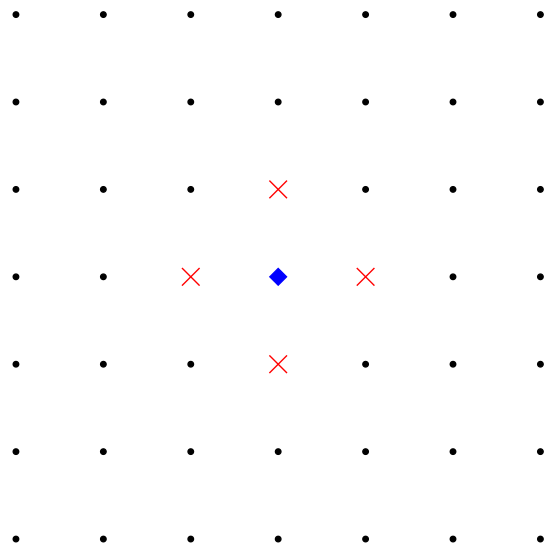
\includegraphics{neighbors_4}} \hspace{0.25in} \resizebox{!}{1.5in}{\includegraphics{neighbors_8}}
\caption{Left: The digital plane. Middle: $4$-neighbors of a point. Right: $8$-neighbors of a point.}
\label{F:Digital_plane}
\end{center}
\end{figure}

A natural start to building a digital topology might be to identify neighborhoods. The idea of a neighborhood is to consider elements that are close to a point, and in the digital world there are different ways to do this. Given a point $(x,y)$ in $\Z^2$, the 4-neighbors of $(x,y)$ are the points vertically or horizontally adjacent to $(x,y)$: that is, the points $(x \pm 1, y)$ and $(x, y \pm 1)$. The 8-neighbors of $(x,y)$ are the 4-neighbors along with the points diagonally adjacent to $(x,y)$: that is, $(x \pm 1, y)$, $(x, y \pm 1)$, $(x \pm 1, y \pm 1)$. These neighbors are illustrated in Figure \ref{F:Digital_plane}, with the crosses indicating the neighbors of the highlighted point. 

In the continuous case, we define a path between points to be a continuous function from $[0,1]$ to the space. However, we cannot have continuity in the digital world. So we define paths by moving through neighbor points. That is, if $k$ is either $4$ or $8$, a $k$-path is a finite sequence $p_0$, $p_1$, $\ldots$, $p_m$ in $\Z^2$ such that $p_1$ is a $k$-neighbor of $p_2$, $p_2$ is a $k$-neighbor of $p_3$, $\ldots$, $p_{m-1}$ is a $k$-neighbor of $p_m$.  

\begin{activity} \label{act:digital_graph_theory} ~
\ba

\item Show that there is a $4$-path connecting any two points in $\Z^2$. Then explain why there is an $8$-path connecting any two points in $\Z^2$. 


\item In the continuous case, every Jordan curve separates $\R^2$ into two connected regions. To have a similar theorem in the discrete case, we need a notion of connectedness in $\Z^2$. Every image is made up of a finite number of pixels, and so we can think of a digital image as existing in a finite subspace of $\Z^2$. Since connectedness and path connectedness are equivalent in finite topological spaces, we us the idea of $k$-paths to define connectedness in $\Z^2$. We say that a subset $S$ of $\Z^2$ is $k-connected$ if if any two of its points can be joined by a $k$-path in $S$. 

Figure \ref{F:Digital_curves} show two sets (curves) in the digital plane indicated by the points that connect the line segments (examples taken from A Topological Approach to Digital Topology, T. Yung Kong,  R. Kopperman, and P. Meyer, \emph{American Mathematical Monthly}, 98 (1991), no. 10, 901-917). Let $S_1$ be the set illustrated at left in Figure \ref{F:Digital_curves} and $S_2$ the set at right. 
\begin{figure}[h]
\begin{center}
\resizebox{!}{2.0in}{\includegraphics{digital_curve_1}} \hspace{0.5in} \resizebox{!}{2.0in}{\includegraphics{digital_curve_2}}
\caption{Sets $S_1$ (left) and $S_2$ (right) in the digital plane.}
\label{F:Digital_curves}
\end{center}
\end{figure}

Is $S_1$ $4$ connected? Is $S_1$ $8$ connected? Verify your answer. Repeat with $S_2$. 

\item We can now define a Jordan $k$-curve to be a finite $k$-connected set which contains exactly two $k$-neighbors
for each of its points.

Is $S_1$ a Jordan $4$-curve? Is $S_1$ a Jordan $8$-curve? Verify your answer. Repeat with $S_2$. 

\item As usual, we define a component to be a maximal connected set. Explain why $S_1$ is a Jordan $8$-curve whose complement is connected and why $S_2$ is a Jordan $4$-curve whose complement consists of three connected $4$-components. This example shows that there is no Jordan curve theorem in digital topology using the standard notions of $k$-connectedness with $k$ either $4$ or $8$. So neither 4-adjacency nor 8-adjacency provides an analogue of the Jordan curve theorem and it is necessary to use a combination of both. That is, a Jordan $4$-curve with at least five points separates $\Z^2$ into exactly two $8$-components, and a Jordan $8$-curve with at least five points separates $\Z^2$ into exactly two $4$-components. 

\ea

\end{activity}

\begin{comment}

\ActivitySolution

\ba

\item Let $(a,b)$ and $(c,d)$ be points in $\Z^2$. Let $p_0 = (a,b)$. Let $p_i = (a \pm i,b)$ for $0 \leq i \leq |c-a|$, with a plus if $a \leq c$ and a minus if $a > c$. Then $p_t$ is a $4$-neighbor of $p_{t-1}$ for each $t$. Then let $p_{j+|c-a|} = (c, b \pm j)$ for $0 \leq j \leq |d-b|$ with a plus if $b \leq d$ and a minus if $b > d$. Then the sequence $p_s$ with $0 \leq s \leq |c-a| + |b-d|$ is a $4$-path from $(a,b)$ to $(c,d)$. The fact that every $4$-neighbor is an $8$-neighbor means that there is also an $8$-path between any two points in $\Z^2$. 

\item Notice that no two points in $S_1$ can be connected by a $4$-path in $S_1$. So $S_1$ is not $4$-connected. However, any two points in $S_1$ can be connected by an $8$-path, so $S_1$ is $8$-connected. Since any two points in $S_2$ are $4$ connected by a $4$-path in $S_2$ (and hence connected by an $8$-path in $S_2$), it follows that $S_2$ is both $4$ and $8$-connected. 

\item Since $S_1$ is not $4$-connected, $S_1$ in not a Jordan $4$-curve. Note that $S_1$ contains exactly two $8$-neighbors for each of its points and so $S_1$ is a Jordan $8$-curve. The set $S_2$ contains exactly two $4$-neighbors for each of its points and so $S_2$ is a Jordan $4$-curve. However, $S_2$ contains four $8$-neighbors of the point $p$, as illustrated in Figure \ref{F:Digital_curves_P}, so $S_2$ is not a Jordan $8$-curve.  
\begin{figure}[t]
\begin{center}
\resizebox{!}{2.0in}{\includegraphics{digital_curve_3}} 
\caption{The point $P$ in $S_2$.}
\label{F:Digital_curves_P}
\end{center}
\end{figure}


\item The single point set with the point $O$ at the center of $S_1$ contains no $4$-neighbors of that point, so that single point comprises a component. Any two points in the set $A = \Z^2 \setminus (S_1 \cup \{O\})$ are $4$-connected in $A$, so $\Z^2 \setminus S_1$ has two connected $4$-components. Notice that the point $O$ is $8$-connected to every point in $A$. So there is only one $8$-component of $\Z^2 \setminus S_1$. 

Let $Q_1$ and $Q_2$ be the two points in the ``interior" of $S_2$. Neither $Q_1$ nor $Q_2$ is $4$-connected to any other point in $\Z^2 \setminus S_2$, so $\{Q_1\}$ and $\{Q_2\}$ are two $4$-connected components of $\Z^2 \setminus S_2$. Let $B = \Z^2 \setminus (S_2 \cup \{Q_1\} \cup \{Q_2\})$. Any two points in $B$ are $4$-connected, so $B$ is also a $4$-component of $\Z^2 \setminus S_2$. 

Now $Q_1$ and $Q_2$ are $8$-connected, but neither is $8$-connected to any point in $B$. The set $B$ is $4$-connected, hence $8$-connected, and so $\Z^2 \setminus S_2$ has two $8$-components. 


\ea

\end{comment}

In Activity \ref{act:digital_graph_theory} we discussed the importance of a digital Jordan curve theorem. In the next activity we describe a topology in which such a theorem exists. 

\begin{activity} \label{act:digital_Jordan_curve} Consider $Z$ with the topology $\tau_1$ with basis $\{B(n)\}$, where 
\[B(n) = \begin{cases} \{n\}	&\text{if $n$ is odd}, \\ \{n-1,n,n+1\}	&\text{if $n$ is even}. \end{cases}\]
This topology is called the \emph{digital line topology} or the \emph{Khalimsky topology}\index{topology!Khalimsky} on $\Z$. Notice that all sets of the form $\{n\}$ are open when $n$ is odd. 

\ba

\item Show that any set of the form $\{n\}$ where $n$ is even is closed in the digital line topology. 

\item To define a \emph{Khalimsky topology} on $\Z^2$ we use the product topology.  Explain why the collection of sets $\{B(m,n)\}$ where 
\[B(m,n) = \begin{cases} \{(m,n)\}  & m \text{ and } n \text{ odd,} \\
\{(m-i,n-j) \mid -1 \leq i \leq 1, -1 \leq j \leq 1\} &m \text{ and } n \text{ even,} \\
\{(m,n-1), (m,n), (m,n+1)\} &m \text{ odd and } n \text{ even,} \\
\{(m-1,n), (m,n), (m+1,n)\} &m \text{ even and } n \text{ odd} 
\end{cases}\]
is a basis for the Khalimsky topology $\tau_2$ on $\Z^2$. (This topology was originally published by  E. Khalimsky in \emph{Applications of connected ordered topological spaces in topology}, Conference of math. departments of Povolsia, 1970.)

\item New we want to define a digital Jordan curve. Our first step is to define a \emph{digital path}. Recall that a path in a topological space is a homeomorphism from the interval $[0,1]$ into the space. So we need the concept of a digital interval. If $z_1 < z_2$ in $(\Z, \tau_1)$, the \emph{digital interval} $[z_1,z_2]$ is the set
\[[z_1, z_2] = \{z \in \Z \mid z_1 \leq z \leq z_2\}.\]
The integers $z_1$ and $z_2$ are called the \emph{endpoints} of the digital interval $[z_1,z_2]$.  

\begin{definition} Let $X$ be a topological space.
\begin{itemize}
\item A \textbf{digital path}\index{digital path} in $X$ is the range of a continuous function from a digital interval to $X$.
\item A \textbf{digital arc}\index{digital arc} in X is the range of a homeomorphism from a digital interval to $X$.
\end{itemize}
\end{definition}

Let 
\begin{align*}
S_1 &= \{(1,-1), (1,1), (-1,1), (-1,-1)\}, \\
S_2 &= \{(0,0), (1,-1), (2,0), (1,1)\}, \text{ and } \\
S_3 &= \{(1,-1), (1,0), (1,1), (0,1), (-1,1), (-1,0), (-1,-1), (0,-1)\}.
\end{align*}
Show that $S_1$ is not a digital path but $S_2$ and $S_3$ are digital paths.  

\item To produce a digital Jordan Curve Theorem, we need a definition of a digital Jordan curve. 

\begin{definition} A \textbf{digital Jordan curve}\index{digital Jordan curve} is a finite connected set $J$ with $|J| \geq 4$ such that $J \setminus \{j\}$ is a digital arc for each $j \in J$.
\end{definition}

So every digital Jordan curve is a connected set. Show that any finite digital path in $\Z^2$ is a connected set. (Hint: Is every digital interval connected?)

\item The upshot of all of this is the following theorem (a proof can be found in A Topological Approach to Digital Topology, T. Yung Kong,  R. Kopperman, and P. Meyer, \emph{American Mathematical Monthly}, 98 (1991), no. 10, 901-917).

\begin{theorem} \label{thm:digital_Jordan_curve} If $J$ is a digital Jordan curve in the digital plane $\Z^2$, then $\Z^2 \setminus J$ has exactly two components. 
\end{theorem}

The two components in Theorem \ref{thm:digital_Jordan_curve} split the digital plane into an infinite region (the outside) and a finite region (the inside). 

Show that $S_2$ is a digital Jordan curve (and thus splits $\Z^2$ into two connected components). 

\ea

\end{activity}

\begin{comment}

\ActivitySolution

\ba

\item Let $n$ be an even integer. Then 
\[\Z \setminus \{n\} = \bigcup_{m \neq n} B(m),\]
which is a union of open sets in the digital line topology.

\item A basis for the open sets in $\Z^2$ is found by taking the cross products of basis elements of the topology in $\Z$. 
\begin{itemize}
\item If $m$ and $n$ are both odd, then
\[B(m,n) = B(m) \times B(n) = \{m\} \times \{n\} = \{(m,n)\}.\]

\item If $m$ and $n$ are both even, then
\[B(m,n) = B(m) \times B(n) = \{m-1,m,m+1\} \times \{n-1, n, n+1\} = \{(m-i,n-j) \mid -1 \leq i \leq 1, -1 \leq j \leq 1\}.\]

\item If $m$ is odd and $n$ is even, then
\[B(m,n) = B(m) \times B(n) = \{m\} \times \{n-1, n, n+1\} = \{(m,n-1), (m,n), (m,n+1)\}.\]

\item If $m$ is even and $n$ is odd, then
\[B(m,n) = B(m) \times B(n) = \{m\} \times \{n-1, n, n+1\} = \{(m-1,n), (m,n), (m+1,n)\}.\]

\end{itemize}

This makes $\{B(m,n)\}$ a basis for the Khalimsky topology on $\Z^2$.

\item Suppose $I = [a_1,a_2,a_3, a_4]$ is a digital interval. The nontrivial open sets in the subspace topology on $I$ are the sets $\{a_1\}$, $\{a_3\}$, $\{a_1,a_2,a_3\}$, $\{a_3,a_4\}$, $\{a_1,a_3\}$, and $\{a_1,a_3,a_4\}$ if $a_1$ is odd and $\{a_2\}$, $\{a_3\}$, $\{a_1,a_2\}$, $\{a_2,a_3, a_4\}$, $\{a_2,a_3\}$, and $\{a_1,a_2,a_3\}$ if $a_1$ is even.  The single point sets $\{(1,-1)\}$, $\{(1,1)\}$, $\{(-1,1)\}$, and $\{(-1,-1)\}$ are all open in the subspace topology on $S_1$, so the subspace topology on $S_1$ is the discrete topology. Suppose there is a bijection $f: I \to S_1$, and let $x = f(a_2)$ if $a_1$ is odd and $x = f(a_1)$ if $a_1$ is even. Then $f^{-1}(\{x\})$ is not open in $I$ and $f$ is not continuous. Therefore, $S_1$ is not a digital path. 

Let $P_1 = (0,0)$, $P_2 = (1,-1)$, $P_3 = (2,0)$, and $P_4 = (1,1)$. Define $f: [0,3] \to S_2$ by $f(i) = P_{i+1}$. By construction, $f$ is a bijection. The nontrivial open sets in the subspace topology on $[0,3]$ are the sets $\{0,1\}$, $\{1\}$, $\{1,2,3\}$, $\{3\}$, $\{0,1,3\}$, and $\{1,3\}$. The nontrivial open sets in the subspace topology on $S_2$ are $\{P_1, P_2, P_4\}$, $\{P_2\}$, $\{P_2, P_3, P_4\}$, $\{P_4\}$, $\{P_2,P_4\}$. Since
\begin{align*}
f^{-1}(\{P_1,P_2,P_4\}) &= \{0,1,3\} \\
f^{-1}(\{P_2\}) &= \{1\} \\
f^{-1}(\{P_2,P_3,P_4\}) &= \{1,2,3\} \\
f^{-1}(\{P_4\}) &= \{3\} \\
f^{-1}(\{P_2,P_4\}) &= \{1,3\} 
\end{align*}
we conclude that $f$ is a continuous function. So $S_2$ is a digital path. 

Finally, we turn to $S_3$. Let $P_1 = (1,-1)$, $P_2 = (1,0)$, $P_3 = (1,1)$, $P_4 =  (0,1)$, $P_5 = (-1,1)$, $P_6 = (-1,0)$, $P_7 = (-1,-1)$, and $P_8 = (0,-1)$. A basis for the open sets in $S_3$ is 
\[\{\{P_1\}, \{P_1,P_2,P_3\}, \{P_3\}, \{P_3,P_4,P_5\}, \{P_5)\}, \{P_5,P_6,P_7\}, \{P_7\}, \{P_7,P_8,P_1\}\}.\]

Let $I = [1,2,3,4,5,6,7,8]$. A basis for the open sets in $I$ is 
\[\{\{1\}, \{1,2,3\}, \{3\}, \{3,4,5\}, \{5\}, \{5,6,7\}, \{7\}, \{7,8\}\}.\]

Define $f: I \to S_3$ by $f(i) = P_i$. Now
\begin{align*}
f^{-1}(\{P_1\}) &= \{1\} \\
f^{-1}(\{P_1,P_2,P_3\}) &= \{1,2,3\} \\
f^{-1}(\{P_3\}) &= \{3\} \\
f^{-1}(\{P_3,P_4,P_5\}) &= \{3,4,5\} \\
f^{-1}(\{P_5\}) &= \{5\} \\
f^{-1}(\{P_5,P_6,P_7\}) &= \{5,6,7\} \\
f^{-1}(\{P_7\}) &= \{7\} \\
f^{-1}(\{P_7,P_8,P_1\}) &= \{7,8,1\} 
\end{align*}
all of which are open in $S_2$. Thus, $f$ is a continuous function from $I$ to $S_2$. Also,
\begin{align*}
f(\{1\}) &= \{P_1\} \\
f(\{1,2,3\}) &= \{P_1,P_2,P_3\} \\
f(\{3\}) &= \{P_3\} \\
f(\{3,4,5\}) &= \{P_3,P_4,P_5\} \\
f(\{5\}) &= \{P_5\} \\
f(\{5,6,7\}) &= \{P_5,P_6,P_7\} \\
f(\{7\}) &= \{P_7\} \\
f(\{7,8\}) &= \{P_7,P_8\} 
\end{align*}

\item Let $I = [a_1,a_2, \ldots, a_n]$ with $n \geq 4$ be a digital interval and suppose that $I$ is disconnected. Then there is a separation $U$ and $V$ of $I$. Suppose $a_1 \in U$. Let $k$ be the smallest integer such that $a_k \notin U$. Then $a_k \in V$. We consider the cases $a_k$ odd and $a_k$ even.
\begin{itemize}
\item Suppose $a_k$ is odd. The only basic open set that contains $a_{k-1} \in U$ is the set $\{a_{k-2}, a_{k-1}, a_k\}$. Since $U$ is a union of basic open sets, it follows that $\{a_{k-2}, a_{k-1}, a_k\} \subseteq U$. But then $U \cap V \neq \emptyset$ and $U$ and $V$ do not form a separation of $I$.
\item Suppose $a_k$ is even. But then $\{a_{k-1}, a_{k}, a_{k+1}\} \subseteq V$ and again $U \cap V \neq \emptyset$.
\end{itemize}
We conclude that no separation of $I$ exists and so $I$ is connected. 

Since a digital path is the continuous image of a connected set, any digital path is connected. 

\item As a digital path, we know that $S_2$ is connected. 

\begin{itemize}
\item Consider $J_1 = S_2 \setminus \{(0,0)\} = \{(1,-1), (2,0), (1,1)\}$. Let $P_1 = (1,-1)$, $P_2 = (2,0)$, and $P_3 = (1,1)$. Let $I = [1,2,3]$ and define $f: I \to J_1$ by $f(i) = P_i$. The nontrivial open sets in $J_1$ are $\{P_1\}$,$\{P_3\}$, and $\{P_1, P_3\}$ while the nontrivial open sets in $I$ are $\{1\}$, $\{3\}$, and $\{1,3\}$. Now
\begin{align*}
f^{-1}(\{P_1\}) &= \{1\} \\
f^{-1}(\{P_3\}) &= \{3\} \\
f^{-1}(\{P_1,P_3\}) &= \{1,3\} 
\end{align*}
and
\begin{align*}
f(\{1\}) &= \{P_1\} \\
f^(\{3\}) &= \{P_3\} \\
f(\{1,3\}) &= \{P_1,P_3\}. 
\end{align*}
So $f$ is a homeomorphism and $J_1$ is a digital arc.

\item Consider $J_2 = S_2 \setminus \{(1,-1)\} = \{(0,0), (2,0), (1,1)\}$. Let $P_0 = (0,0)$, $P_1 = (1,1)$, and $P_2 = (2,0)$. Let $I = [0,1,2]$ and define $f: I \to J_2$ by $f(i) = P_i$. The nontrivial open sets in $J_2$ are $\{P_0,P_1\}$,$\{P_1\}$, and $\{P_1, P_2\}$ while the nontrivial open sets in $I$ are $\{0,1\}$, $\{1\}$, and $\{1,2\}$. Now
\begin{align*}
f^{-1}(\{P_0,P_1\}) &= \{0,1\} \\
f^{-1}(\{P_1\}) &= \{1\} \\
f^{-1}(\{P_1,P_2\}) &= \{1,2\} 
\end{align*}
and
\begin{align*}
f(\{0,1\}) &= \{P_0,P_1\} \\
f^(\{1\}) &= \{P_1\} \\
f(\{1,2\}) &= \{P_1,P_2\}. 
\end{align*}
So $f$ is a homeomorphism and $J_2$ is a digital arc.

\item Consider $J_3 = S_2 \setminus \{(2,0)\} = \{(0,0), (1,-1), (1,1)\}$. Let $P_1 = (1,-1)$, $P_2 = (0,0)$, and $P_3 = (1,1)$. Let $I = [1,2,3]$ and define $f: I \to J_1$ by $f(i) = P_i$. The nontrivial open sets in $J_1$ are $\{P_1\}$,$\{P_3\}$, and $\{P_1, P_3\}$. Now
\begin{align*}
f^{-1}(\{P_1\}) &= \{1\} \\
f^{-1}(\{P_3\}) &= \{3\} \\
f^{-1}(\{P_1,P_3\}) &= \{1,3\} 
\end{align*}
and
\begin{align*}
f(\{1\}) &= \{P_1\} \\
f^(\{3\}) &= \{P_3\} \\
f(\{1,3\}) &= \{P_1,P_3\}. 
\end{align*}
So $f$ is a homeomorphism and $J_3$ is a digital arc.

\item Finally, consider $J_4 = S_2 \setminus \{(1,1)\} = \{(0,0), (1,-1), (2,0)\}$. Let $P_0 = (0,0)$, $P_1 = (1,-1)$, and $P_2 = (2,0)$. Let $I = [0,1,2]$ and define $f: I \to J_4$ by $f(i) = P_i$. The nontrivial open sets in $J_4$ are $\{P_0,P_1\}$,$\{P_1\}$, and $\{P_1, P_2\}$. Now
\begin{align*}
f^{-1}(\{P_0,P_1\}) &= \{0,1\} \\
f^{-1}(\{P_1\}) &= \{1\} \\
f^{-1}(\{P_1,P_2\}) &= \{1,2\} 
\end{align*}
and
\begin{align*}
f(\{0,1\}) &= \{P_0,P_1\} \\
f^(\{1\}) &= \{P_1\} \\
f(\{1,2\}) &= \{P_1,P_2\}. 
\end{align*}
So $f$ is a homeomorphism and $J_4$ is a digital arc.

\end{itemize}

We conclude that $S_2$ is a digital Jordan curve. 


\ea

\end{comment}


Digital Jordan curves, as described in Activity \ref{act:digital_Jordan_curve}, are important in order to have a digital Jordan curve theorem. Christer O. Kiselman presents the following theorem to characterize digital Jordan curves in \emph{Discrete Geometry for Computer Imagery}, Springer-Verlag, 2000, p. 46-56. 

\begin{theorem} \label{thm:digital_curve} A subset $J$ of $\Z^2$ equipped with the Khalimsky topology is a digital Jordan curve if and only if $J = \{P_1, P_2, \ldots, P_m\}$ for some even integer $m \geq 4$ and for all $j$, $P_{j?1}$ and $P_{j+1}$ and no other points are adjacent to $P_j$; moreover each path consisting of three consecutive points $P_{i?1}$, $P_i$, $P_{i+1}$ turns at $P_i$ by $45^{\circ}$ or $90^{\circ}$ or not at all if $P_i$ is a pure point, and goes straight ahead if $P_i$ is mixed.
\end{theorem}

We investigate this theorem in the next activity.

\begin{activity} ~
\ba
\item We need to first define the appropriate terms. Let $X$ be a topological space. Two points $x$ and $y$ in $X$ are \emph{adjacent} if $x \neq y$ and the set $\{x, y\}$ is connected. Then let $N(x)$ to be the intersection of all neighborhoods of $x$. 

Show that distinct elements $x$ and $y$ in a topological space $X$ are adjacent if and only if $x \in N(y)$ or $y \in N(x)$. 

\item A point $(x_1,x_2)$ in $\Z^2$ is called \emph{pure} if $x_1$ and $x_2$ have the same parity. Otherwise, the point is \emph{mixed}. Find $N(P)$ if $P$ is a pure point or a mixed point.

\item In Activity \ref{act:digital_Jordan_curve} we show that the set $S_1 = \{(1,-1), (1,1), (-1,1), (-1,-1)\}$ is not a digital path and so not a digital Jordan curve. Which part of Theorem \ref{thm:digital_curve} does $S_1$ violate? 

\item In Activity \ref{act:digital_Jordan_curve} we show that the set $S_2 = \{(0,0), (1,-1), (2,0), (1,1)\}$ is a digital Jordan curve. Show that in $S_2$, the property from Theorem \ref{thm:digital_curve} that $x_{j-1}$ and $x_{j+1}$ and no other points are adjacent to $x_j$ is satisfied for each $j$.


\ea

\end{activity}

\begin{comment}

\ActivitySolution

\ba
\item Suppose $x$ and $y$ are adjacent. Then $\{x,y\}$ is connected. Suppose $x \notin N(y)$. We will show that $y \in N(x)$. There is a neighborhood $M$ of $y$ such that $x \notin M$. It follows that there is an open set $V$ in $M$ with $y \in V$ and $x \notin V$. Let $N$ be a neighborhood of $x$ and let $U \subset N$ with $x \in U$. Since $\{x,y\} \subseteq U \cup V$ and $\{x,y\}$ is connected, it must be the case that $U \cap V \neq \emptyset$. The fact that $x \notin V$ implies that $y \in U$. We conclude that $y \in N(x)$. 

Now suppose that $x \in N(y)$ or $y \in N(x)$. Without loss of generality, assume that $x \in N(y)$. To show that $\{x,y\}$ is connected, proceed by contradiction and assume that there is a separation $U$, $V$ of $\{x,y\}$ with $x \in U$ and $y \in V$. But $V$ is a neighborhood of $y$ and so $x \in N(y) \subseteq V$, a contradiction.

\item Let $P = (a,b)$. 
\begin{itemize}
\item Suppose $a$ and $b$ are both odd. Then $\{(a,b)\}$ is a neighborhood of $(a,b)$. It follows that $N((a,b)) = B(a,b)$. 
\item Suppose $a$ and $b$ are both even. Any neighborhood of $P$ must contain a basic open set that contains $P$, and the only such set is $B(a,b)$. So $N(P) = B(a,b)$. 
\item Suppose $a$ is odd and $b$ is even. Any neighborhood of $P$ must contain a basic open set that contains $P$, and the only such sets are $B(a,b)$, $B(a-1,b)$ and $B(a+1,b)$. The intersection of these sets is $B(a,b)$. A similar argument holds if $a$ is even and $b$ is odd. 
\end{itemize}

\item Let $P = (a,b)$ be an element in $S_1$. Then $P$ is pure with both components odd, so $N(P) = B(a,b) = \{P\}$. So none of the other elements in $S_1$ are adjacent to any other element in $S_1$. 

\item We know that $N((-1,1)) = \{(-1,1)\}$, $N((1,1)) = \{(1,1)\}$, $N((0,0)) = \{(-1,-1), (-1,0), (-1,1), (0,-1), (0,0), (0,1), (1,-1), (1,0), (1,1)\}$, and $N((2,0)) = \{(1,-1), (1,0), (1,1), (2,-1), (2,0), (2,1), (3,-1), (3,0), (3,1)\}$. We see therefore that $(0,0)$ and $(2,0)$ are adjacent to $(1,-1)$, but $(1,1)$ is not adjacent to $(1,-1)$. Also, $(1,-1)$ and $(1,1)$ are adjacent to $(2,0)$, but $(0,0)$ is not adjacent to $(2,0)$.  

\ea

\end{comment}



